\chapter{Lecture 3}

%--- 信息 ----
\begin{center}
    讲师:王立威 \qquad
    课程时间:25.Mar.4th \qquad 
    笔记:25.June.7th
\end{center}

\bigskip

考虑一般的$p$进制编码(经典比特为$p=2$进制,但也有3进制计算机)此时,随机元$X$的熵为 
\[
H(X) := \sum_{i=1}^n p_i \log_p 1/p_i
\]
相应地,这个量的单位也应该从bit变为其他的单位. 

上节课说到均匀分布时熵最大,可以总结成如下命题
\begin{proposition}
    对于$X = (m_1, \dots, m_n)$,那么$H(X) \le \log_2 n$
\end{proposition}
\begin{proof}
    使用Jensen不等式即可,此略.
\end{proof}

事实上,熵的定义非常符合直觉,我们通过一个例子感受 
\begin{example}
    我们考虑随机变量$X,Y,Z$. $X$有分布列$(p_1,\dots, p_n)$,其中$p_n = q_1 + q_2$;$Y$的分布列正比于$(q_1, q_2)$;$Z$有分布列$p_1,\dots, p_{n-1}, q_1, q_2$. 

    可以写成如下形式:
    \[
    \begin{matrix}
        X: & p_1 & p_2 & \cdots & p_n(= & q_1 + q_2) \\
        Y: & \ & \ & \ & \dfrac{q_1}{q_1 + q_2} & \dfrac{q_2}{q_1 + q_2}  \\
        Z: & p_1 & p_2 & \cdots & q_1 & q_2
    \end{matrix}
    \]

    此时$H(X),H(Y),H(Z)$满足什么关系?
\end{example}
\begin{solution}
    应该满足$H(X) + p_n\cdot H(Y) = H(Z)$,下面通过计算来说明.
    \begin{align*}
        & H(Z) - H(X) \\
        = & \ \left[
            \sum_{i=1}^{n-1} p_i \log_2 1/p_i + \sum_{j=1}^2 q_j \log_2 1/q_j
        \right] - \left[
            \sum_{i=1}^{n-1} p_i \log_2 1/p_i + 
            p_n \log_2 1/p_n
        \right] \\
        = & \ \sum_{j=1}^2 q_j \left(
            \log 1/q_j - \log_2 1/p_n
        \right) \\
        = & \ \sum_{j=1}^2 q_j \log_2\dfrac{q_1 + q_2}{q_j} \\
        = & \ p_n \sum_{j=1}^2 \dfrac{q_j}{q_1 + q_2} \log_2\dfrac{q_1 + q_2}{q_j} = p_n \cdot H(Y)
    \end{align*}

    通过上面的例子,我们发现熵的定义十分合理.$Y$可以视作对于$X$在$m^{(X)}_n$的情况下的进一步阐释(细化);而$Z$直接融合了$X$和$Y$对其的阐释.阐释发生的概率是$p_n$,所以$Z$的信息量就是$X$的信息量加上$p_n$倍$Y$的信息量.
\end{solution} 

以上结论对于$\boldsymbol{q}$是更高维的情况下也成立,称作\textbf{熵的加性}. 

我们至此讨论了熵的定义和性质,但回归到实际实践当中,我们当然需要$l_i$全部为整数.换言之,对于随机变量$X$服从分布列$P=(p_1,\dots, p_n)$,我们想要构造一个具体的编码算法,得到平均码长最短的实际编码$C = (c_1, \dots, c_n)$,称\textbf{最优码}. 以下,我们记$c_i$的长度为$\abs{c_i}$

可以得到最优码的一些性质:
\begin{itemize}
    \item 如果$p_1 \ge p_2 \ge \cdots \ge p_n$,那么对于最优码一定有$\abs{c_1} \le \abs{c_2} \le \cdots \le \abs{c_n}$ 
    \item Kraft不等式取等条件成立: $\sum_{i=1}^n 2^{-\abs{c_i}} = 1$ 
    \item 如果$p_1 \ge p_2 \ge \cdots \ge p_n$,那么会有$\abs{c_n} = \abs{c_{n-1}}$. (直观而言,这是在说二叉树中$c_n$一定会有兄弟;数学而言,这是为了满足上一条性质的等号要求)
    \item 若$(c_1, \dots, c_n)$是$(p_1,\dots, p_n)$的最优码,那么$(c_1, \dots, \tilde{c}_{n-1})$是$(p_1,\dots, p_{n-1}+p_n)$的最优码.其中我们假定$c_{n-1}, c_n$在二叉树中是兄弟,仅有最后一位不同,而$\tilde{c}_{n-1}$代表它们二者前面的公共前缀.(该性质可通过反证法得出)
\end{itemize}

结合这些性质便可以设计算法,逐步将问题的维度降低.这个算法就是Huffman编码(自行查阅该算法,此不介绍). 

接下来拓展一下熵的定义,对于多个变量可定义联合熵. 
\begin{definition}[联合熵]
    对于两个随机变量$X,Y$,联合分布列为$P_{X,Y} = (p_{i,j})$,定义\textbf{联合熵}(joint entropy)为 
    \[
    H(X, Y) := \sum_{i,j} p_{i,j} \log_2 1/p_{i,j}
    \]
\end{definition}

可见这样的定义和原本熵的定义很类似,意义是将$X,Y$一起编码时的最短平均码长;$X,Y$一共的信息量等等. 

\begin{theorem}
    对于两个随机变量$X,Y$,有$H(X,Y) \le H(X) + H(Y)$,取等当且仅当$X,Y$独立.
\end{theorem}

\begin{example}
    取$X=Y$,可以发现$H(X, Y) = H(X) \le 2H(X) = H(X) + H(Y)$
\end{example}

类似地,可以定义条件熵
\begin{definition}[条件熵]
    对于两个随机变量$X,Y$,对于$X$的可能取值$x_i$(满足$\Pr[X = x_i] > 0$),定义 
    \[
H(Y|X=x_i) := \sum_{j} \Pr[Y=y_j | X = x_i] \log_2 \dfrac{1}{\Pr[Y=y_j | X = x_i]}
    \]

    总体的\textbf{条件熵}(conditional entropy)就定义为 
    \[
H(Y|X) := \sum_{i} \Pr[X = x_i] H(Y|X=x_i)
    \]
\end{definition} 

以下定理说明条件熵$H(Y|X)$的意义为“$Y$在$X$的基础上引入的新信息”:
\begin{theorem}
    对于两个随机变量$X,Y$,有 
    \[
    H(X,Y) = H(X) + H(Y|X) = H(Y) + H(X|Y)
    \]
\end{theorem}

% \begin{figure}[H]
%     \centering
%     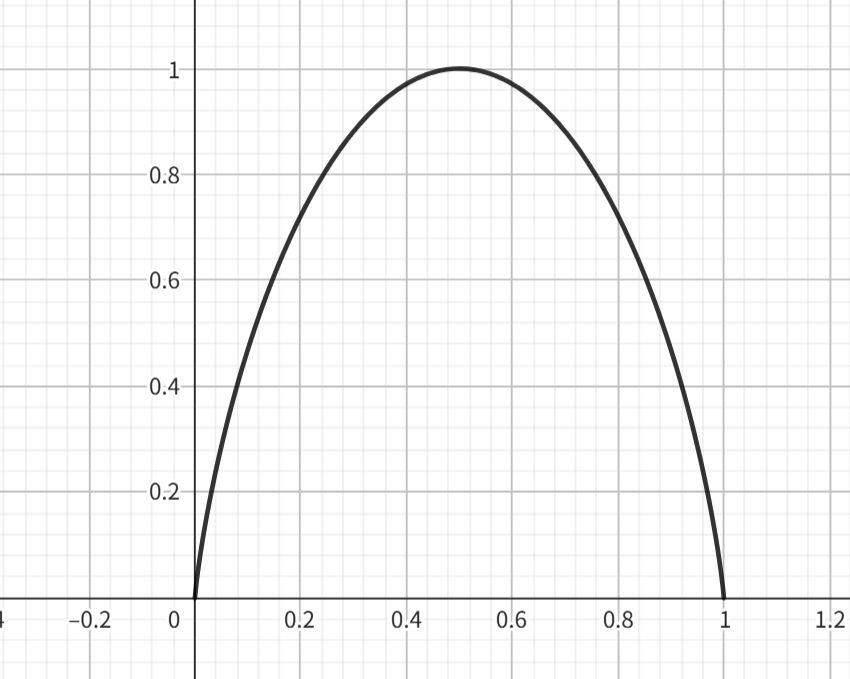
\includegraphics[width=.6\textwidth]{images/c2_1.png}
%     \caption{$H=x\log 1/x + (1-x)\log 1/(1-x)$的图像}
% \end{figure}